
\section{Simultaneous Localization And Mapping}
Esta sección describe los conocimientos básicos respecto a la Localización y Mapeo Simultáneos (SLAM), a la vez de introducir parte de los algoritmos y sensores mencionados en secciones anteriores.

\subsection{Introducción al SLAM}
El problema de localización y mapeo simultáneos (SLAM) se basa en el proceso de un robot que construye un mapa de su entorno desconocido (\textit{mapping}) mientras este lo explora conociendo su ubicación en el mismo (\textit{localization}). Dicho problema puede ser expresado como el dilema del huevo o la gallina, ya que para conocer la ubicación del robot, es necesario determinar el mapa que lo rodea, sin embargo, para que el mismo pueda estimar el mapa en el cual se encuentra, necesita primero conocer su ubicación dentro de ese entorno. 

A partir de la detección y seguimiento de marcas naturales del ambiente (\textit{landmarks}), las técnicas de SLAM  estiman  tanto  la  posición  del  robot  como  la  ubicación  de las marcas en el entorno. El mapa se construye con las estimaciones de las posiciones  de  dichas  marcas,  las  cuales  van  siendo ajustadas  a  medida  que  son observadas desde distintas posiciones. Es necesario que la localización sea precisa, ya que si la misma es inexacta generará problemas a la hora de reconstruir el mapa. Es por esto que el mapeo y la localización dependen uno del otro, y se ejecutan \textit{simultáneamente} de forma entrelazada.

El SLAM es un problema difícil ya que, debido al ruido de los sensores utilizados, ninguna de las mediciones es perfecta. Esto significa que ni el movimiento del robot ni la estructura del entorno se conocen de manera absolutamente precisa, sino solo hasta cierto grado de incertidumbre. Con el fin de hacer frente a estas incertidumbres, el SLAM generalmente se entiende y se aborda mediante técnicas y modelos probabilísticos. Las diferentes formas en que se representan las funciones de densidad probabilística constituyen las diferencias en cada enfoque. 
\textbf{MIRAR LO COMENTADO}
% Muchas de ellas utilizan filtros de Bayes, tal como lo es el Filtro de Kalman Extendido (EKF) 
% \begin{large}
% [DURRANT-WHYTE2006]
% [KALMAN1960]
% \end{large}, o en versiones más modernas, por ejemplo, el Fast-SLAM
% \begin{large}
% [PONER FASTSLAM BIEN]
% \end{large}. 
Sin embargo, el uso de enfoques de estimación de estado para describir el problema de SLAM implica resolver una serie de inconvenientes que se generan a partir del mismo, siendo de los más destacados la \textit{asociación de datos}\textbf{[ref 103 y 104 de reid2016]} y el \textit{cierre de ciclo}.

\subsubsection{Asociación de datos}
Uno de los problemas comunes dentro del SLAM corresponde a la asociación de datos (\textit{data asociation}), el cual es el proceso de asociar los datos de los sensores utilizados con las características del ambiente, generando de esta forma los landmarks. En otras palabras, se busca asociar la medición del sensor con alguno de los \textit{n} landmarks ya extraídos y, en caso de que no pertenezca a ninguno de ellos, se generará un landmark nuevo \textit{n+1}. Es importante poder discernir de cuál landmark se trata o si es en efecto uno nuevo, ya que debido al ruido inherente de los sensores puede que caiga entre dos de ellos, como puede observarse en la Figura \ref{fig:dataassociation}, haciendo que pueda tender equívocamente al incorrecto, o creer que no se tiene dicho landmark cuando en realidad era uno ya medido.

\begin{figure}[!ht]
    \centering
    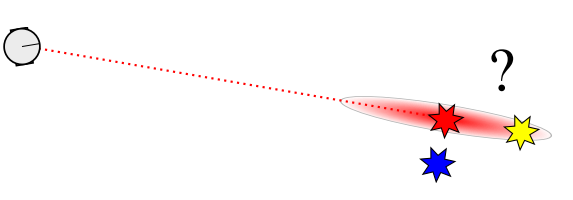
\includegraphics[width=\textwidth]{Img/DataAssociation.png}
    \caption{El problema de la asociación de datos: dificultad de discernir si el landmark detectado (rojo) corresponde a alguno de los ya existentes, o si en realidad es uno del que no se tuvo registro anteriormente}
    \label{fig:dataassociation}
\end{figure}

\subsubsection{Online SLAM y full SLAM}
Los mapas SLAM se construyen a partir de millones de lecturas de sensores, que se comparan entre sí en un paso de asociación de datos que depende completamente de las estimaciones de pose actuales. Para este caso, en el que tanto la pose como el mapa se expresan sólo en base a las mediciones del paso de tiempo actual, el problema se lo conoce como \textit{online SLAM} y se expresa mediante el posterior
% \bm{p}_t es la pose y m el mapa. z es la medicion y u la variable de control
% seria el maximum likelihood?
\begin{equation}
    p(\bm{p},\bm{m}|\bm{y}_{0:t},\bm{u}_{0:t})
\end{equation}
siendo $\bm{p}$ la pose, $\bm{m}$ el mapa, $\bm{y}$ las mediciones y $\bm{u}$ las variables de control.

En cambio, la evaluación y la reevaluación de estas asociaciones de datos, al mismo tiempo que se calcula y actualiza \textit{todo el historial} de poses del robot, describe el problema de \textit{full SLAM} \textbf{[ref 6 de reid2016]}
\begin{equation}
    p(\bm{p}_{0:t},\bm{m}|\bm{y}_{0:t},\bm{u}_{0:t})
\end{equation}

Si bien este último no puede resolverse para entornos no triviales, los enfoques descritos en la literatura a menudo producen resultados útiles en entornos del mundo real. En concreto, con el fin de reducir la complejidad del algoritmo se toman como supuestos comunes que el \textit{entorno es estático}, es decir, que el mapa no varía con el tiempo, y por segundo que las trayectorias de los robots \textit{pueden predecirse}, logrando así que los modelos de movimiento puedan predecir dónde es probable que esté un robot, permitiendo que la búsqueda de asociaciones de datos comience cerca del óptimo global.

\subsubsection{Cierre de ciclo}
\textbf{[REFS DE REID Y VER CASTRO]}
Si bien lo que se busca es evitar errores principalmente de localización, debido al ruido inherente de los sensores utilizados como se mencionó anteriormente, los algoritmos de SLAM no pueden estimar exactamente tanto la ubicación del robot como el mapa que lo rodea, sino hasta con cierto grado de incertidumbre. Como se ejecuta el algoritmo de manera secuencial, el error se irá acumulando a través del tiempo, resultando en una pésima estimación luego de varias corridas. Una forma de poder mitigar en parte estos errores es mediante el reconocimiento de una posición en la que el robot ya estuvo anteriormente. Tomar conocimiento de que se ha efectuado un ciclo en la trayectoria permite calcular el error cometido en la estimación de la posición y da origen a una serie de procesos que permiten corregir tanto la localización actual del robot como el mapa hasta ese momento construido. Este reconocimiento se lo conoce como \textit{cierre de ciclo} (\textit{loop closure}), el cual puede verse en la Figura \ref{fig:poseloopclcorr}.


\begin{figure}[!ht]
    \centering
    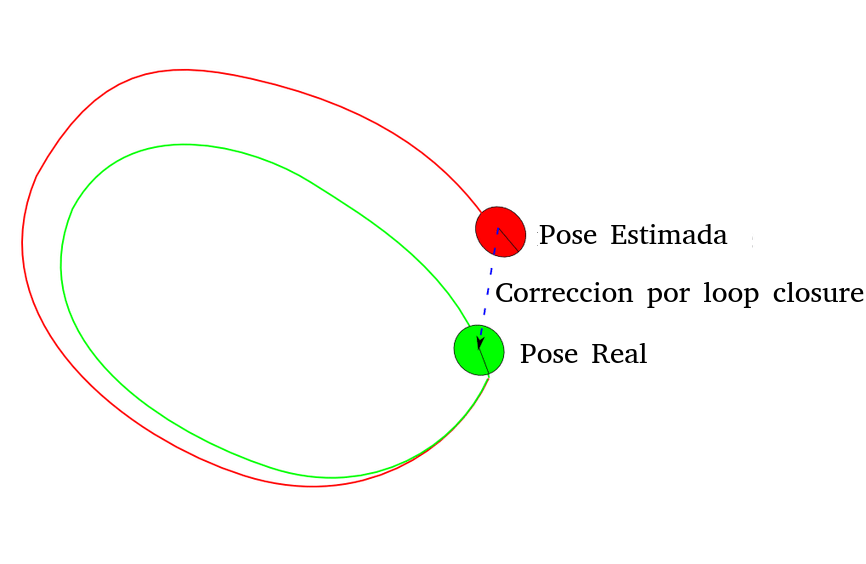
\includegraphics[width=\textwidth]{Img/Pose_LoopClosureCorr.png}
    \caption{Estimación de pose y su correción mediante el loop closure}
    \label{fig:poseloopclcorr}
\end{figure}

\subsection{Mapas}
\textbf{DE Suenderhauf 2012}
En base a los sensores extereoceptivos utilizados además del entorno en el que se encuentran los robots y tareas que tengan que realizar, los mapas creados pueden variar considerablemente. \textbf{THRUN 2002, SICILIANO 2008, THRUN 2005}

\subsubsection{Occupancy Grid Maps}
El concepto de esta técnica es la de discretizar el ambiente a mapear, utilizando pequeñas celdas o regiones discretas $m_i$, como puede observarse en la Figura \ref{fig:occupancygridmaps}.a. A cada una de estas celdas se le asocia un valor que expresa la probabilidad
\begin{equation}
    p(m_i|\bm{y}_{0:t},\bm{x}_{0:t})
\end{equation}
de que dicha celda esté ocupada por un obstáculo, dados todos los datos de los sensores hasta el momento ($\bm{y}_{0:t}$) y todas las poses del robot ($\bm{x}_{0:t}$). En caso de que se desconozca el valor de dichas celdas, el valor por defecto de las mismas es de 0.5. 

\begin{figure}[!ht]
    \centering
    \subfloat[Representación de cada celda en base a si la misma se encuentra ocupada, libre o no se tiene información al respecto]{{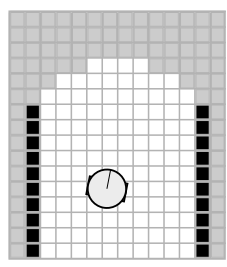
\includegraphics[width=0.45\textwidth]{Img/OccupancyGrids.png}}}%
    \qquad
    \subfloat[Mapa generado por un LIDAR]{{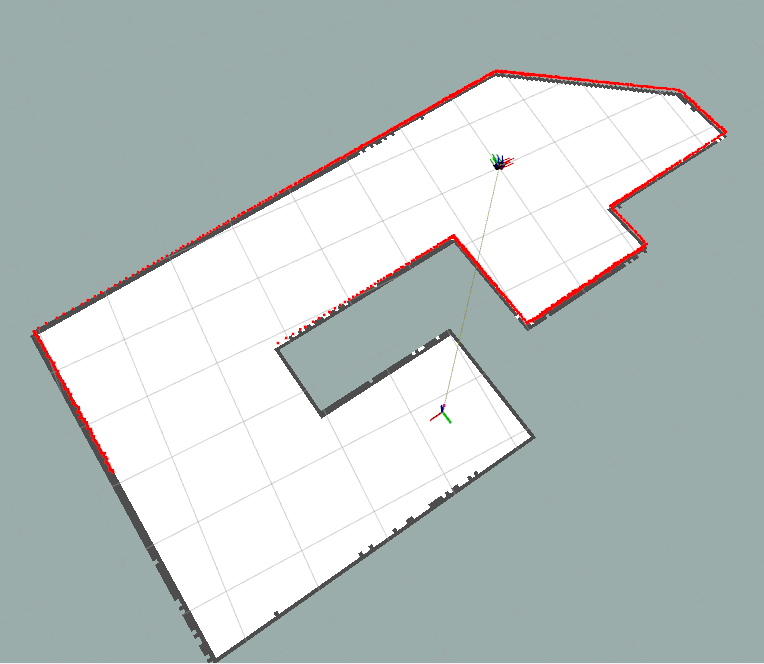
\includegraphics[width=0.45\textwidth]{Img/LIDAROccupancyGridMap.png}}}%
    \caption{Occupancy Grid Maps}
    \label{fig:occupancygridmaps}
\end{figure}


Un ejemplo de un mapa generado por un LIDAR 2D puede observarse en la Figura \ref{fig:occupancygridmaps}.b, donde los cuadros blancos corresponden a celdas libres, los negros a las ocupadas y, las grises, a las que no se tiene información alguna. A su vez, estos mapas pueden llevarse a la espacio tridimensional para representar datos provenientes de, por ejemplo, LIDAR 3D o cámaras.

\subsubsection{Mapas de características}
A diferencia de los Occupancy Grid Maps, los cuales generan un mapa denso del ambiente, los \textit{mapas de características} contienen sólo la posición de distintos landmarks o características del ambiente, resultando en un mapa disperso. Un ejemplo del mismo puede verse en la Figura \ref{fig:dataassociation} \textbf{O PONGO OTRA IMG?}. Dependiendo del principio de medición del sensor que recolecta estos landmarks, existen diferentes tipos de ellos
\begin{itemize}
    \item \textit{El Rango y el rumbo} se conocen, tal como es el caso de las cámaras estéreo o las cámaras RGB-D, en el que la ubicación del landmark respecto al sensor se encuentra bien definida, resultando ser el más sencillo de los tres tipos. En la Figura \ref{fig:landmarktypes}.a puede observarse al mismo.
    \item \textit{Sólo el rango} es conocido, como se observa en la Figura \ref{fig:landmarktypes}.b, haciendo que sea necesario triangular, por ejemplo, para la señal de WiFi, entre la fuerza de la señal recibida de diferentes routers y así conseguir la ubicación del robot en base a estos.
    \item \textit{Sólo el rumbo} es conocido, observado en la Figura \ref{fig:landmarktypes}.c, como es el caso de las cámaras monoculares, haciendo difícil medir la profundidad de cada punto.
\end{itemize}

\begin{figure}[!ht]
    \centering
    \subfloat[Se tiene rango y rumbo]{{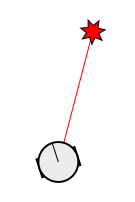
\includegraphics[width=0.3\textwidth]{Img/LandmarkRangeBearing.png}}}%
    \qquad
    \subfloat[Se tiene sólo el rango]{{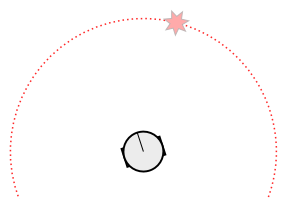
\includegraphics[width=0.3\textwidth]{Img/LandmarkRange.png}}}%
    \subfloat[Se tiene sólo el rumbo]{{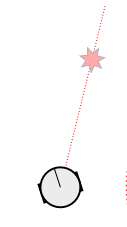
\includegraphics[width=0.3\textwidth]{Img/LandmarkBearing.png}}}%
    \caption{Tipos de landmarks}
    \label{fig:landmarktypes}
\end{figure}

\subsubsection{Grafos de pose}
Los grafos de pose representan la trayectoria del robot como una estructura grafos donde los nodos representan las poses del robot y los bordes entre los nodos representan las conexiones espaciales entre estas poses. Los bordes contienen, por ejemplo, información de odometría o expresan cierres de ciclo. En la Figura puede verse el esquema de un grafo de pose, donde la trayectoria del robot es representada por los grafos donde los nodos son las poses del robot en un punto concreto de tiempo.
\begin{figure}[!ht]
    \centering
    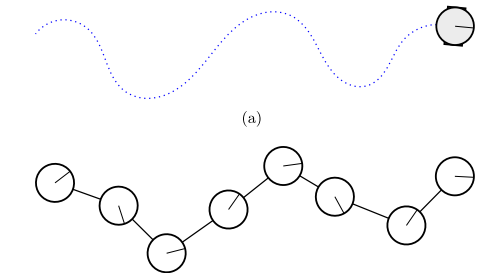
\includegraphics[width=\textwidth]{Img/PoseGraphStructure.png}
    \caption{Esquema de un grafo de pose}
    \label{fig:posegraphstructure}
\end{figure}

Si bien los landmarks explícitos u otra información sobre el medio ambiente no son parte del grafo de pose en sí, dicha información se puede adjuntar a los nodos en el grafo, lo que permite que el grafo de pose exprese occupancy grids en 2D o 3D o mapas de características y cualquier combinación de ellos.

\ifimagenes
\else
\subsection{Algoritmos de SLAM}
Puede decirse que un algoritmo de SLAM consiste en tres operaciones básicas, las cuales se repiten en cada paso de tiempo
\begin{itemize}
    \item El robot se mueve por el entorno, hasta alcanzar un nuevo punto de vista de la escena, que debido al ruido inherente de los sensores ocasiona que aumente la incertidumbre en la localización del mismo.
    \item El robot descubre landmarks en el ambiente, los que requieren ser incorporados al mapa.
    \item El robot observa el mapa que fue mapeado anteriormente y lo utiliza para corregir tanto la localización de dicho landmark como la del propio robot.
\end{itemize}

Si bien existen numerosos algoritmos para realizar el problema de SLAM, a continuación se describen algunos de los enfoques principales que se encuentran en la literatura respecto al tema en cuestión.

\subsubsection{EKF-SLAM}
El enfoque del EKF para solucionar el problema de SLAM se trata de un problema orientado al online SLAM mediante el uso de datos de sensores recopilados a partir del movimiento y la rotación del robot. Esto se puede hacer, por ejemplo, utilizando encoders y una IMU. Además, también es necesario recopilar información del entorno mediante, por ejemplo, el uso de un LIDAR. Con estos datos, el algoritmo realiza un seguimiento del lugar donde probablemente se ubica el robot dentro de un mapa, así como un seguimiento de los puntos de referencia específicos observados. Es por esto que se utiliza un mapa de características para este caso.

Al considerar un mapa estático, el único factor variante en el tiempo es el movimiento del robot. Por lo tanto, se tienen diferentes comportamientos para cada parte del vector de estados. El mismo en este caso se define como
\begin{equation}
    \bm{x} = 
    \begin{bmatrix}
        \bm{p} \\
        \bm{\mathcal{M}}
    \end{bmatrix}
\end{equation}
donde $\bm{p}$ corresponde a la pose del robot\footnote{Por lo general se suele incorporar la velocidad, ya que se utilizan las ecuaciones de la física clásica. Para la orientación puede utilizarse la forma de cuaterniones mediante la Expresión (\ref{eq:edoquaternion}).} y $\bm{\mathcal{M}}=(\mathcal{L}_1,...,\mathcal{L}_n)$ corresponde a los estados de los landmarks, siendo $n$ la cantidad de ellos detectados. En base a este, el resto de los parámetros del filtro de Kalman Extendido se modificarán respecto al visto en la Sección \ref{sec:stateestimation}\textbf{[SOLA 2014]}. Puede verse que a medida que el mapa aumenta, el costo computacional se incrementará, ya que se tendrán cada vez más landmarks.

Además de la complejidad cuadrática, este filtro cuando se aplica al problema SLAM tiene como desventaja sustancial \textbf{[Csorba 1997 DE SU - FAST-SLAM]}
la sensibilidad a fallas que presenta en las asociaciones de datos. Este problema con el EKF se aplica en situaciones en las que se desconocen las asociaciones de datos. El EKF mantiene una única hipótesis de asociación de datos por observación, típicamente elegida usando una heurística de máxima verosimilitud. Si la asociación de datos elegida por esta heurística es incorrecta, el efecto de incorporar esta observación en el EKF nunca se puede eliminar.

\subsubsection{FastSLAM}


\subsubsection{GraphSLAM}
Utilizando un grafo de poses, el GraphSLAM se orienta a un problema de full SLAM que consta de dos restricciones. Primero, necesita de datos de odometría (que suelen ser las entradas de control $\bm{u}$) que conecten los estados de las poses $\bm{x}_k$ y $\bm{x}_{k+1}$ como puede ser mediante los datos de un LIDAR o la odometría propia de los encoders
\begin{equation}
    \bm{x}_{k+1} \sim \mathcal{N}(f(\bm{x}_{k},\bm{u}_k),\bm{R}_k)
\end{equation}
donde $\bm{\Sigma}_k$ corresponde a la matriz covarianza en el paso de tiempo $k$.

Segundo, para poder detectar un cierre de ciclo, dos poses, que pueden no ser contiguas, se conectan mediante una Gaussiana,
\begin{equation}
    \bm{x}_j \sim \mathcal{N}(f(\bm{x}_k,\bm{c}_{kj}), \bm{Q}_{kj})
\end{equation}
siendo $\bm{c}_{kj}$ el cierre de ciclo.

La solución para este tipo de SLAM se basa en el método del máximo a posteriori (MAP), siendo $\bm{x}^*$ el punto donde la distribución tiene su máximo
\begin{equation}
    \bm{x}^* = argmax_x\ p(\bm{x}|\bm{u})
\end{equation}

Siendo que tanto la odometría como el cierre de ciclo cuentan con distribuciones Gaussianas independientes, el posterior puede factorizarse como
\begin{equation}
    p(\bm{x}|\bm{u},\bm{c}) \propto \underbrace{\prod_k p(\bm{x}_{k+1}|\bm{x}_{k},\bm{u}_k)}_{\text{\parbox{10em}{\centering Restricciones de odometría}}}\ \underbrace{\prod_{kj}p(\bm{x}_j|\bm{x}_k,\bm{c}_{kj})}_{\text{\parbox{10em}{\centering Restricciones de cierres de ciclo}}}
\end{equation}
que, aplicando el logaritmo como en la Expresión (\ref{eq:mlewithlog}), y teniendo en cuenta la analogía con los cuadrados mínimos ponderados
\begin{align}
    \bm{x}^* &= argmax_x\ p(\bm{x}|\bm{u},\bm{c}) \\
    &= argmin_x\ -log(\bm{x}|\bm{u},\bm{c}) \\
     &= argmin_x\ \bm{e}_k^T\bm{R}_k^{-1}\bm{e}_k + \bm{e}_{kj}^T\bm{Q}_{kj}\bm{e}_{kj} \\
     &= argmin_x\ \underbrace{\sum_{i} ||f(\bm{x}_i,\bm{u}_i)-\bm{x}_{i+1})||^2_{\bm{R}_i}}_{\text{{\centering Restricciones de odometría}}} + \underbrace{\sum_{kj} ||f(\bm{x}_i,\bm{c}_{kj}) - \bm{x}_{j}||^2_{\bm{Q}_{kj}}}_{\text{{\centering Restricciones de cierres de ciclo}}}
\end{align}
siendo $||a-b||^2_{\bm{O}} = (a - b)^T\bm{O}^{-1}(a-b)$ la definición de la distancia Mahalanobis. Esta puede minimizarse con algunas de las regresiones vistas en la Sección \ref{sec:regressionanalysis}, dependiendo de la morfología de la señal $f$.

\begin{huge}
ESTE ES QUE EL QUE USO!!!
\end{huge}

\fi